\documentclass[10pt,twocolumn,letterpaper]{article}

\usepackage{statcourse}
\usepackage{times}
\usepackage{epsfig}
\usepackage{graphicx}
\usepackage{amsmath}
\usepackage{amssymb}

% Include other packages here, before hyperref.

% If you comment hyperref and then uncomment it, you should delete
% egpaper.aux before re-running latex.  (Or just hit 'q' on the first latex
% run, let it finish, and you should be clear).
\usepackage[breaklinks=true,bookmarks=false]{hyperref}


\statcoursefinalcopy


\setcounter{page}{1}
\begin{document}


%%%%%%%%%%%%%%%%%%%%%%%%%%%%%%%%%%%%%%%%%%%%%%%%%%%%%%%%%%%%%%%
% DO NOT EDIT ANYTHING ABOVE THIS LINE
% EXCEPT IF YOU LIKE TO USE ADDITIONAL PACKAGES
%%%%%%%%%%%%%%%%%%%%%%%%%%%%%%%%%%%%%%%%%%%%%%%%%%%%%%%%%%%%%%%



%%%%%%%%% TITLE
\title{Midterm Project Report for Newspaper Bias project}

\author{Tom Arend\\
{\tt\small t.arend@phd.hertie-school.org}
\and
Nicolai Berk\\
{\tt\small nicolai.berk@gmail.com}
}

\maketitle
%\thispagestyle{empty}


% MAIN ARTICLE GOES BELOW
%%%%%%%%%%%%%%%%%%%%%%%%%%%%%%%%%%%%%%%%%%%%%%%%%%%%%%%%%%%%%%%

%%%%%%%%% ABSTRACT
\begin{abstract}
   Newspapers are one of the most important institutions in contemporary democracies. They have the power to affect voting behaviour, as well as polarise the electorate or motivate them to turn out to vote. Therefore, it is surprising that few papers deploy sate-of-the-art Deep Learning technologies to classify ideological bias in news articles. We apply a transformer neural network to classify party press releases by authorship. This model is then applied and optimised to estimate ideological bias in news articles. We fine-tune and validate the model using op-eds by politicians and compare pre-trained model to a BERT model that was not fine-tuned on party press releases. This approach provides a novel way to train powerful models on political language with scarce training data.\footnote{GitHub repository: \url{https://github.com/nicolaiberk/nlpdl\_project}}
\end{abstract}


%%%%%%%%% BODY TEXT

% \begin{itemize}
% {\color{blue}

% \item Remember that you should \textbf{submit the report}  via Moodle and \textbf{include in the report the link to accessible GitHub repository that contains the code}. Also, \textbf{only one member per team} needs to submit the project material. You must include a link to your GitHub repository for the project as the first footnote on the first page. 

% \item The midterm project report should be {\bf 4 pages long (not counting references), and a maximum 10 references}. The report should contain the sections that are already provided in this paper. It forms the basis of the final report with the same structure. Please check out the text in these sections for further information.

% \item Your midterm milestone will be graded on the following criteria:
% \begin{itemize}
% \item Progress: Has the team made good progress on the project? You should have done approximately half of the work of your project.
% \item As a minimum, your milestone should show that you have setup your data, baseline model code, and evaluation metric, and run experiments to obtain some results (assuming you are doing a typical model-building project). Other than this, `good progress' depends on various factors (e.g., whether your model is implemented from scratch or based on an existing codebase).
% \item Understanding: Does the milestone show a strong understanding of its problem, tasks, methods, metrics, and research context?
% \item Writing quality: Does the milestone clearly communicate what you've done and why, providing the requested information, to an appropriate level of detail (given the page limit)?
% \item You will receive some brief feedback on your milestone. Feedback may contain helpful suggestions for your project (e.g., try a particular method, read a particular paper) and/or warnings about your project plan (e.g., if your plans are too ambitious or not ambitious enough), and how you could improve your technical writing (e.g., adjustments to clarity, level of detail, formatting, use of references).
% \end{itemize}

% \item Technical writing is an important skill in this class, in research, and beyond. It's well worth spending time developing your ability to communicate technical concepts clearly. Here are some resources which might help you improve your technical writing:
% \begin{itemize}
% \item Tips for Writing Technical Papers, Jennifer Widom (\url{https://cs.stanford.edu/people/widom/paper-writing.html}).
% \item Write the Paper First, Jason Eisner (\url{https://www.cs.jhu.edu/~jason/advice/write-the-paper-first.html}).
% \end{itemize}

% \item Here are some other things you can do to improve your technical writing:
% \begin{itemize}
% \item Look carefully at several ML / NLP papers to understand their typical structure, writing style, and the usual content of the different sections. Model your writing on these examples.
% \item Think about the NLP / ML papers you've read (for example, the one you summarised for your proposal). Which parts did you find easy to understand and why? Which parts did you find difficult to understand and why? Can you identify any good writing practices that you could use in your technical writing?
% \item Ask a friend to read through your writing and tell you if is clear. This can be useful even if the friend does not have the relevant technical knowledge.
% \end{itemize}
% }
% \end{itemize}

\section{Proposed Method}



% This section details your approach(es) to the problem. For example, this is where you describe the architecture of your model, and any other key methods or algorithms.

% You should also describe your baseline(s). Depending on space constraints, and how standard your baseline is, you might do this in detail, or simply refer the reader to some other paper for the details. 

% If any part of your approach is original, make it clear (so we can give you credit!). For models and techniques that aren't yours, provide references.

% If you're using any code that you didn't write yourself, make it clear and provide a reference or link. When describing something you coded yourself, make it clear (so we can give you credit!).

The measurement of ideology and political bias are the subject of much research on political texts \cite{Bilbao-Jayo2018, Laver2003, Simoes2020}. Despite significant advances in our understanding and detection of ideology, most researchers still face significant constraints when working with text. Notably, they face a lack of appropriately labeled training data. This is linked to the high costs incurred by manually annotating a significant number of speeches, texts, or sentences. It might therefore be useful to infer ideology from other sources of text and apply them to the desired text using transfer learning.\\

We conduct experiments with differently fine-tuned deep learning models to understand if and how transfer learning can be used to measure bias in the absence of abundant training data. To test this, we fine-tune a deep neural network to predict the authoring political party of German press releases. This approach is useful, as political parties represent the major organisers and navigation points for political ideology. The resulting model will then be used to estimate the bias of newspaper articles by assessing the similarity to a political party. In addition, we plan to compare between models that were fine-tuned with different data to assess the effectiveness of this additional fine-tuning step. While the application of transformers to measure bias is not entirely new in political science \cite{Terechshenko2020, Vig2020}, we move beyond the current state-of-the-art by measuring the precise implications of different fine-tuning procedures. \\

Beyond testing the effectiveness of this two-step fine-tuning process, this project will develop a state-of-the-art deep learning model for the measurement of political bias in newspaper articles.  Newspapers represent an important institution in the political world, affecting phenomena ranging from polarization to voter turnout. Much like the shadows in Plato's allegory of the cave, news provide elites and citizens with a representation of a reality they are not able to see themselves \cite{Plato520a}. Given this important role, we believe it worthy to develop a state-of-the-art deep learning model. If existing approaches \cite{Gentzkow2010, Widmer2020} to classify newspaper slant can be improved upon, or even just complemented, we could provide an additional tool for researchers to study the impact of newspaper slant. A working state-of-the-art model might even renew interest in the subject matter and encourage researchers to find new and exciting applications for it. \\

Outside of academia, a confident and robust classifier of newspaper bias might help readers to identify when they are reading an article that is overly partisan. This would perhaps encourage them to approach certain news sources with more scepticism and hold news outlets to higher editorial standards. In the long run, the highlighting of biases in articles might counteract the worrying polarization of entire electorates. \\

We propose to identify newspaper slant by fine-tuning a pretrained transformers model on party press releases before using transfer learning to apply that model to a range of newspaper articles. We measure newspaper bias as an article's similarity to a given party's communication. Using pretrained BERT neural network models for German language\footnote{Link to the model page: \url{https://huggingface.co/transformers/model_doc/distilbert.html}}, we compare how three different training processes affect model performance. We expect optimal performance from a transformer neural network that was fine-tuned in two steps. First we use the pretrained model to classify party press releases by issuing party. Secondly, the model is applied in its actual domain to estimate ideological bias in news articles. We fine-tune and subsequently validate the model using op-eds by politicians. These articles have the advantage of carrying party labels allowing transfer of the categories from the initial fine-tuning process (first step) to the outcome of interest. We compare this fine-tuned model to a BERT model that was not fine-tuned on party press releases and one that was not fine-tuned on newspaper data. This leaves us with three models:

\begin{enumerate}
    \item A model only fine-tuned on newspaper articles authored by politicians.
    \item A model only fine-tuned on party press releases.
    \item A model both fine-tuned on press releases and politicians' newspaper contributions.
\end{enumerate}

This way, we can assess by how much model performance is improved upon, when including information from both party press releases and newspaper data, compared to fine-tuning processes excluding this information.\\

\section{Experiments}

\paragraph{Data:} In this project, we draw on three distinct data sources:\\
\begin{itemize}
    \item A dataset of over 40,000 German party press releases issued between 2010 and 2019, collected by the SCRIPTS project\footnote{\url{https://www.scripts-berlin.eu/index.html}. Special thanks go to Lukas Stötzer for the effortless (for us) provision of the data.}.
    \item A collection of over 2 million German newspaper articles from six major newspapers, published between 2013 and 2019, collected by one of the authors in a previous project (\cite{Krause2021}).
    \item A collection of German newspaper articles authored by politicians collected as part of this project (collectio underway).
\end{itemize}

\paragraph{Evaluation method:} So far, we have successfully fine-tuned a BERT-model to classify party-press releases by authorship (model 2, serving as the basis for model 3). The performance of this model is shown in \ref{fig:party}. As the reader can see, the model performs at a very high, near-perfect level. We believe that the classification performance made hyper-parameter optimisation somewhat obsolete. We are nevertheless open to tweak hyperparameters if the need arises and time permits it. The impressive performance was rather surprising to the authors and shifted the initial focus of the project away from improving the classification of party press releases to the comparison of improvements in the two-step fine-tuning process. Thus, the comparison and improvement of different models applied for the estimation of newspaper slant will be our main focus going forward.\\

\begin{figure}
    \centering
    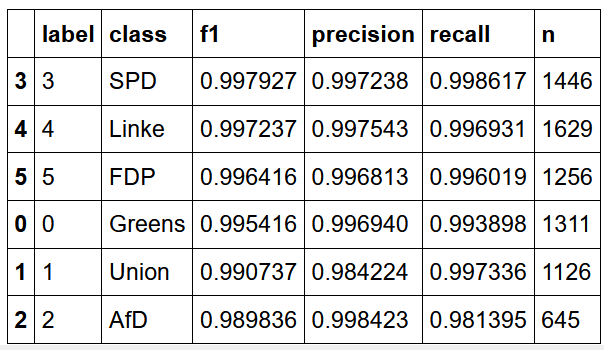
\includegraphics[width=0.4\textwidth]{reports/midterm-report-latex/figures/party_class.png}
    \caption{Performance of model 2 for the classification of party press releases.}
    \label{fig:party}
\end{figure}

For the final assessment of classifier performance, we will use a unique, newly collected set of politicians' op-eds and interviews. This data enables us to compare the impact of different fine-tuning processes (using party press releases, newspaper articles, or both) on model performance, as the outcome categories (authorship party) are identical. We aim for a balance of precision and recall, and will therefore evaluate the models' F1-scores. Additionally, we will assess generalisability by assessing the placement of newspapers - left-wing newspapers such as the TAZ should be placed closer to left-wing parties (Grüne, SPD, Linke) than right-wing newspapers (FAZ, WELT).\\

\paragraph{Experimental details:} 

% How you ran your experiments (e.g. model configurations, learning rate, training time, etc.)

We use the 'distilbert-base-german-cased' model from the Huggingface transformer library\footnote{\url{https://huggingface.co/bert-base-german-cased}.} for all three models. This deep-learning model has been trained to solve different classification tasks on 12 GB of German language data, including Wikipedia, legal data, and news. Given the impressive performance on the party press releases, deviation from the default settings for most hyper-parameters was deemed unnecessary thus far. The same applies for the larger but slower 'bert-base-german-cased' model. We decided on three training epochs, a training batch size of 16, and a weight decay of $0.01$ for regularisation. This might change in the future, depending on the model's performance on the newspaper articles.\\

The configuration of our hyperparameters largely follows the defaults and is as follows\footnote{The model's default settings (which we did not change) can be found here: \url{https://huggingface.co/distilbert-base-german-cased/blob/main/config.json}.}:
\begin{itemize}
    \item Training epochs: $3$
    \item Batch size: $16$
    \item We apply a weight decay as a form of regularisation: $0.01$
    \item Maximum sequence length (longer articles were truncated): $512$
    \item Dropout for each layer: $10\%$
\end{itemize}

\paragraph{Results:} We classified a training set of 4,000 newspaper articles using model 2 (fine-tuned on party press releases). We expected articles from conservative newspapers FAZ and Welt to be more similar to Union and FDP and possibly the AfD, especially compared to the progressive TAZ. Spiegel Online (SPON) is expected to be equally similar to right- and leftwing newspapers.\\

The results can be seen in table \ref{tbl:means}, which shows the average probability for an article to be classified as being authored by a given party. As expected, FAZ and Welt are very similar to Union (81\%) and FDP (58\%/55\%), but also rather similar to the Greens (36\%/35\%). While they show the highest similarity to the AfD (8\%/7\%), similarity to the radical-right party is generally on a very low level among all newspapers. Spiegel Online (SPON) shows lower similarity to the FDP and closer to Union and Greens, but is generally rather similar to the right-wing newspapers. The TAZ shows a comparatively different profile, being very similar to the Greens (average likelihood 70\%), and less similar to the Union parties (41\%), the FDP (32\%), and the AfD (5\%). Surprisingly, it also shows the lowest similarity to the Linke (13\%). Maybe most surprising is the general low similarity to SPD press releases (4\%/5\%). It seems the party has a rather distinctive style in its press releases.\\

\begin{table}[!htbp] \centering 
    \begin{tabular}{@{\extracolsep{1pt}} lcccccc}
    \\[-1.8ex]\hline 
    \hline \\[-1.8ex] 
    Paper & Linke & Grüne & SPD & Union & FDP & AfD \\ 
    \hline \\[-1.8ex] 
    FAZ & $0.15$ & $0.36$ & $0.05$ & $0.81$ & $0.58$ & $0.08$ \\ 
    Welt & $0.15$ & $0.35$ & $0.05$ & $0.81$ & $0.55$ & $0.07$ \\ 
    Spiegel & $0.11$ & $0.39$ & $0.05$ & $0.89$ & $0.34$ & $0.07$ \\ 
    TAZ & $0.13$ & $0.69$ & $0.04$ & $0.41$ & $0.32$ & $0.05$ \\ 
    \hline \\[-1.8ex] 
    \end{tabular} 
  \caption{Mean similarity estimate to each party by newspaper.} 
  \label{tbl:means} 
\end{table}

Given that model 2 is likely the worst performing model, we consider these results to be promising. However, we need to look into the odd performance of the SPD category, which we expected to be similar to SPON articles. As this is not the case, we will need to run a further diagnostics (suggestions are welcome).\\

\section{Future work}

Given the surprisingly good performance of the baseline model on the classification of party press releases, the project can focus on the evaluation of the effectiveness of the two-step fine tuning process as its major contribution. We identified several key tasks to meet this goal;\\

The collection of several hundred newspaper articles and interviews by politicians for fine-tuning and model evaluation is the most important and urgent next step. This will be done mostly by scraping politicians websites within the next week. Once this data is available, we will be able to fine-tune model 1 and model 3 and assess their performance on a held-out set of newspaper articles. The performance and comparison of these new models has become has become the main goal of the project. It will enable us to assess which model performs best, and - more importantly - how much the model is improved upon by each fine-tuning step.\\

Even though the assessment of the models' performance does constitute the major goal of the project, several additional tasks are necessary in order for us to fully grasp the necessary model improvements. Chief among these is the extremely accurate performance of the model 2 when comparing news articles and press releases. We intend to assess this by using a test set that lies in the future, meaning beyond the end-date of the training set currently in use. This way, we can see whether the model's high accuracy owes to idiosyncrasies of party press releases at a given period in time (same topics, same politicians addressed). Should accuracy drop substantially, the model might suffer from overfitting and the classification accuracy might be due to the incorporation of time-specific noise. \\

In the same vein, the surprisingly high misclassification rate among SPON articles and SPD articles will have to be addressed. We will have to see whether this missclassification might also occurr in our two other models. If this should be the case, we would have to focus on structural reasons as to why SPON articles diverge fro our hypothesis. This might entail an in-depth look at the input data. We will most likely take a qualitative approach to understand whether the SPD's press releases are radically different from others or whether the party is really under-represented in the coverage of these newspapers. For now however, we continue under the assumption that the model itself is at fault.  \\

There are some additional tasks that we would like to address should time permit it. Chief among these feature extensive hyper-parameter optimisation to improve the performance of all models. More importantly, we might make additional efforts to understand \textit{why} additional fine-tuning steps could be important (or not). One potential avenue to understand how different fine-tuning processes affect our models, we might build on recent work employing causal mediation analysis to assess the interaction of the structure and predictions in transformer models \cite{Vig2020}.



\section{Conclusion}

Why we changed our focus

{\small
\bibliographystyle{ieee}
\bibliography{bibliography.bib}
}

\end{document}
